ساختار کلی پروتکل بین کلاینت و سرور اینگونه است:

\begin{itemize}

\item 1 بایت مختص packet-type
\item 2 بایت مختص sequence-number
\item 4 بایت مختص checksum 
\item باقی هم برای payload 

\end{itemize}

\subsubsection*{انواع Packet ها}
\textbf{0}: درخواست نام فایل

\textbf{1}: داده

\textbf{2}: ACK

\textbf{3}: ERROR

\textbf{4}: EOF

\textbf{5}: NACK

\subsubsection*{فلوی کار سرور:}
منتظر درخواست است $\longleftarrow$ اگر فایل نبود ERROR می‌فرستد $\longleftarrow$ اگر بود داده‌ها را به بسته‌های کوچک تقسیم و ارسال می‌کند $\longleftarrow$ منتظر ACK یا NACK برای هر بسته $\longleftarrow$ پس از اتمام، EOF می‌فرستد.


\subsubsection*{فلوی کار کلاینت:}
درخواست فایل را می‌فرستد $\longleftarrow$ منتظر دریافت داده می‌ماند $\longleftarrow$ بسته‌ها را با checksum بررسی می‌کند $\longleftarrow$ در صورت درست بودن ACK می‌فرستد، در غیر این صورت NACK $\longleftarrow$ پس از دریافت EOF دانلود تمام می‌شود.

لاگ‌های مرتبط با سرور حین اجرا فایل تست داده شده:

	{
	\centering{
		
		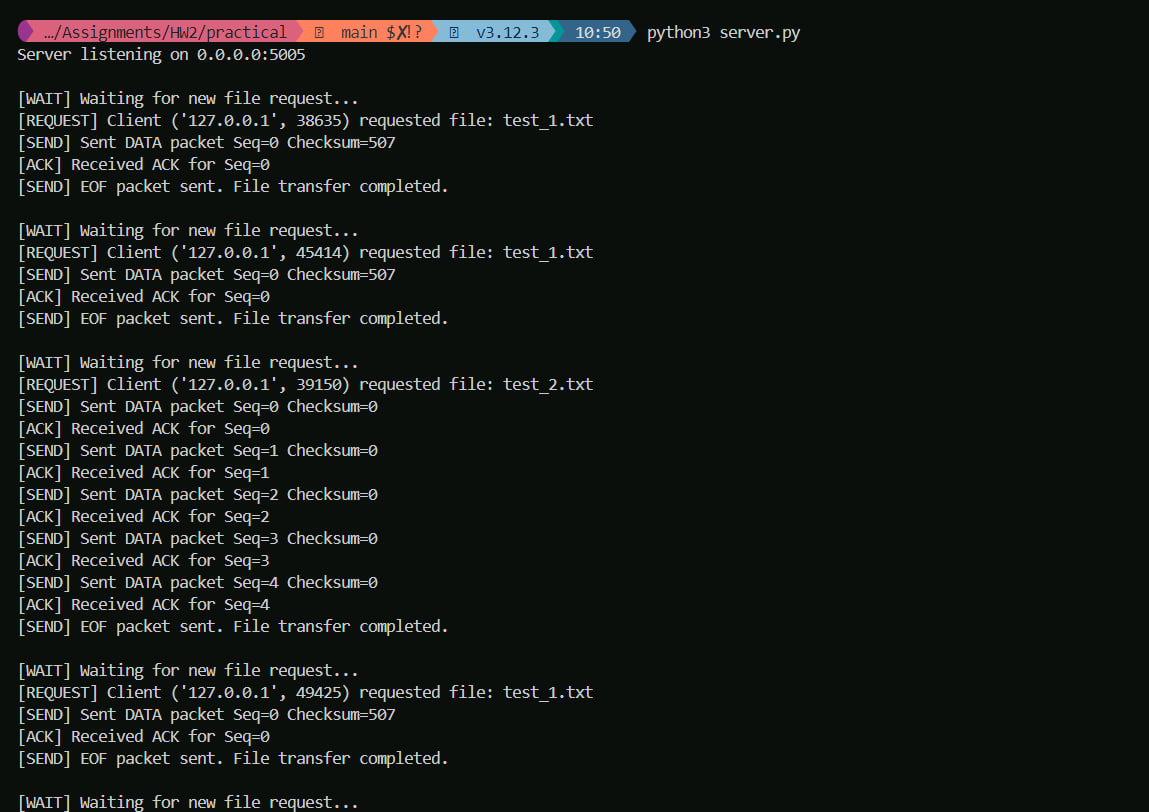
\includegraphics[width=0.7\linewidth]{figs/1}
		
	}
	}


لاگ‌های مرتبط با فایل تست:


		{\centering{
				
				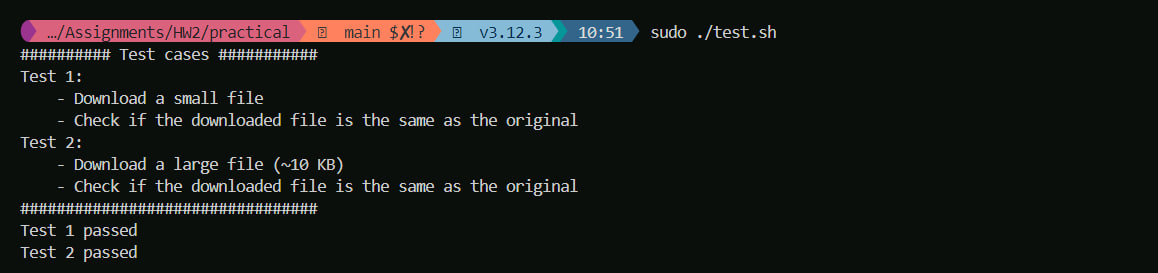
\includegraphics[width=0.7\linewidth]{figs/2}
				
		}}



من برای شبیه‌سازی از دست رفتن بسته‌ها و لینک غیرقابل‌اتکا، داخل کد کلاینت و سرور یک احتمال ثابتی دخیل کردم تا پکت‌ها به مشکل بخورند. سپس آن را روی یک فایل بزرگ‌‌‌تر تست کردم و پکت‌‌های Drop را بررسی کردم که به درستی کار کنند:


{\centering 

{
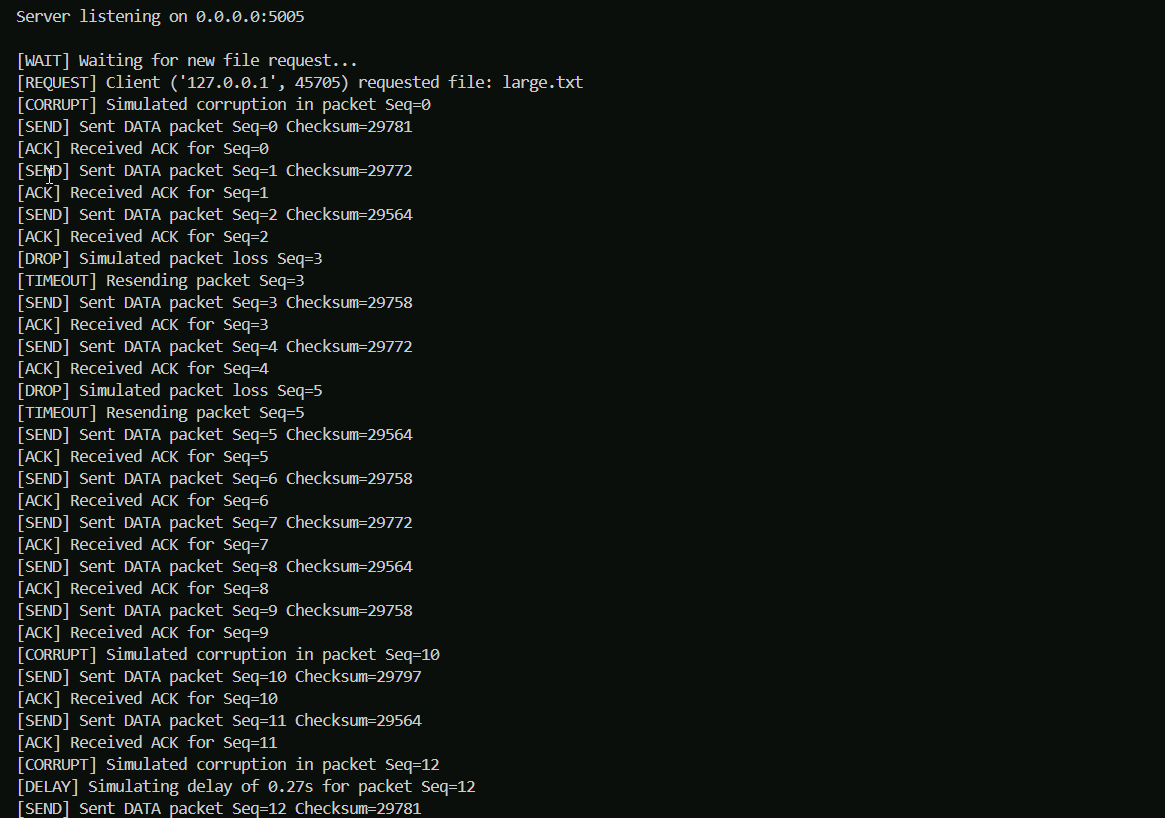
\includegraphics[width=0.7\linewidth]{screenshot001}

}}

همانطور که مشخص است، بعضی از بسته‌ها Drop شده‌اند و seq افزایش نیافته‌است و مجدد ارسال شده است.

همچنین برخی از بسته‌ها Timeout شده‌اند که در عکس لاگ سرور مشخص است. 
در نهایت فایل $large.txt$ به درستی و کامل برای client ارسال شده‌است.

